\section{Resultados Útiles}

En esta sección pondremos demostraciones que son necesarias o útiles para resolver varios problemas.

\subsection{Argumentos de simetría del campo eléctrico}

Para todas las demostraciones de simetría es necesario tener una distribución uniforme de carga e indicar, inicialmente al menos, de manera gráfica por que existe la simetría. Para cada demostración se hará uso de las coordenadas con la que es más fácil trabajar las figuras, pero aplica para todas las coordenadas haciendo las transformaciones pertinentes.

\subsubsection{En esferas}

\label{SimetríaEsfera}
En esferas el campo eléctrico tiene componente solo en $\hat{r}$ a causa de que los campos generados por cargas cercanas se cancelan entre sí, permitiendo solo la existencia en esa dirección. 

En la figura inferior se observa que los campos $\Vec{E}_2$ y $\Vec{E}_1$ generados por $\Delta q_1$ y $\Delta q_2$ en la dirección $P$ se cancelan entre sí, causando el campo $\Vec{E}_{neto}$ en la dirección radial a $P$.
\begin{figure}[H]
    \centering
    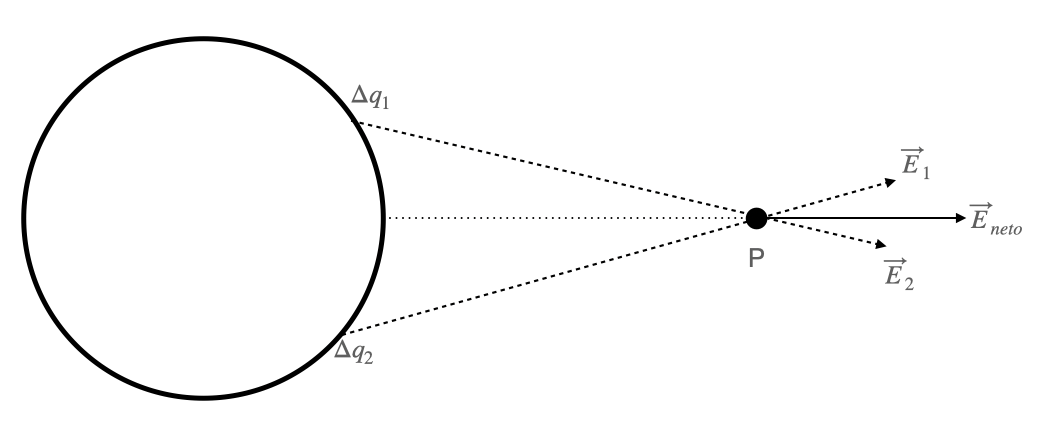
\includegraphics[width=0.7\textwidth]{Resultados_utiles/demost_simetria_esfera.png}
    \label{fig:simetria_esfera}
\end{figure}

\subsubsection{En cilindros infinitos o con altura $\gg$ radio}

\label{SimetríaCilindrosInf}
En cilindros tales que sean de largo infinito o su largo sea mucho mayor ($\gg$) al radio, el campo eléctrico apuntará en la dirección $\hat{\rho}$, esto a que las componentes de los campos en $\hat{z}$ se cancelan entre sí.

En la figura inferior se observa esto, donde en el punto $P$ los campos $\Vec{E}_1$ y $\Vec{E}_2$ generados por $\Delta q_1$ y $\Delta q_2$ se cancelan entre sí dando origen al campo $\Vec{E}_{neto}$ en $\hat{\rho}$.
\begin{figure}[H]
    \centering
    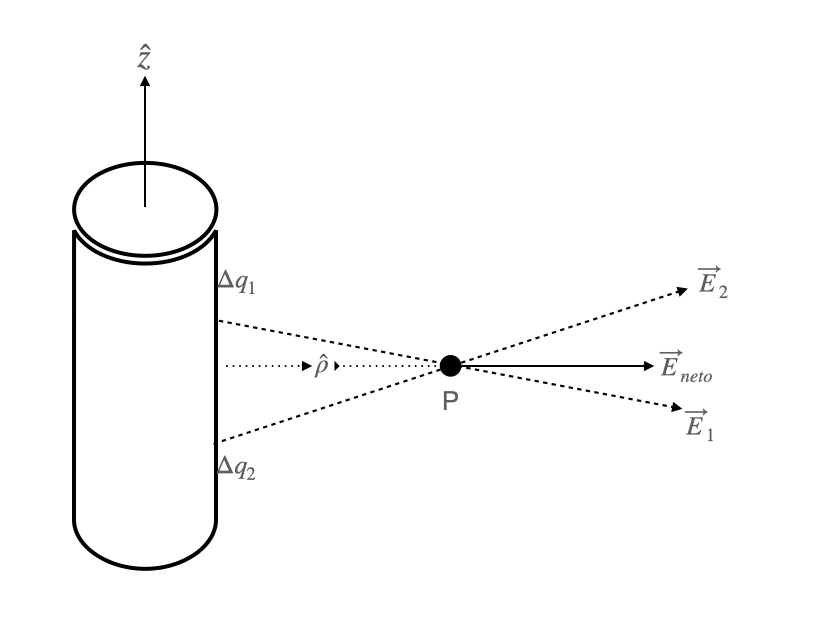
\includegraphics[width=0.7\textwidth]{Resultados_utiles/demost_simetria_cili.png}
    \label{fig:simetria_cilindro}
\end{figure}
\subsubsection{En planos infinitos}
\label{SimetríaPlanosInf}
En planos infinitos o con largo 'muy grande', se tendrá que el campo solo apuntará en la dirección normal a la superficie, esto es a causa de que las componentes en las otras direcciones se cancelan entre sí. 
\medbreak
En la figura inferior se observa esto, donde la normal es $\hat{z}$.
\begin{figure}[H]
    \centering
    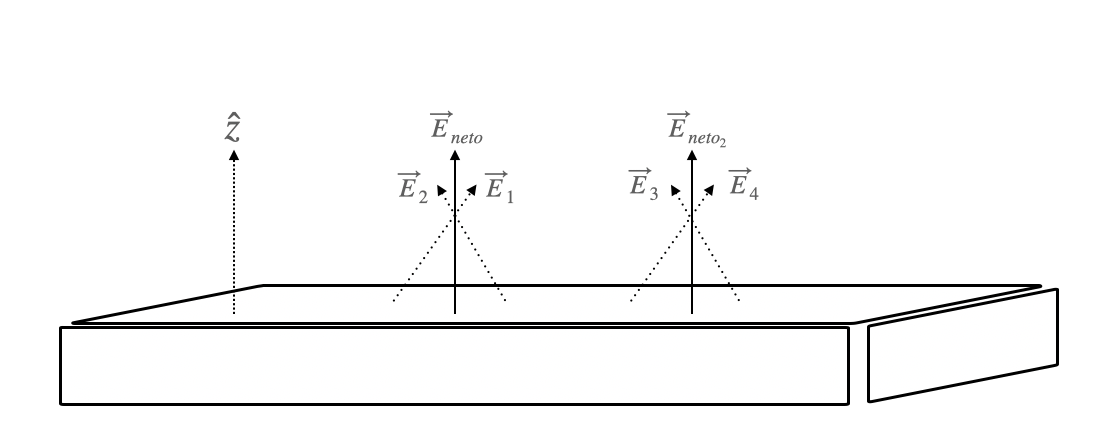
\includegraphics[width=0.7\textwidth]{Resultados_utiles/demost_simetria_plano.png}
    \label{fig:simetria_plano}
\end{figure}
\medbreak
Tomando un punto $r$ arbitrario fuera del plano en el lado donde $z$ es positivo, para todo punto $p$ en el plano, existe $p'$ simétrico a $p$ respecto a la recta perpendicular al plano que pasa por $r$, tal que la suma de los vectores que apuntan de $p$ a $r$ y de $p'$ a $r$ es paralela al eje $z$

\[\Vec{pr} = \Vec{r}-\Vec{p} = (r_x-p_x)\hat{x} + (r_y-p_y)\hat{y} + r_z\hat{z}\]
\[\Vec{p'r} = \Vec{r}-\Vec{p'} = (p_x-r_x)\hat{x} + (p_y-r_y)\hat{y} + r_z\hat{z}\]
\[\Vec{pr}+\Vec{p'r} = 2r_z\hat{z}\]

Con esto, el campo eléctrico en el lado positivo de $z$ depende sólo de $z$

\[\Vec{E_p}(\Vec{z})=E_p(z)\hat{z}\]

El razonamiento es el mismo para el lado negativo de z, con la única diferencia que el campo apunta en sentido opuesto.

\subsection{Ecuación de Poisson para esferas}
\label{PoissonEsferas}
Por simetría el potencial de una esfera depende sólo de la componente $r$ de las coordenadas esféricas.


\[\nabla^2V =
\nabla\cdot\left(\frac{\partial V}{\partial r}\hat{r}\right) =
\frac{1}{r^2}\frac{\partial}{\partial r}\left(\frac{\partial V}{\partial r}r^2\right) =
\frac{\partial^2 V}{\partial r^2}+\frac{2}{r}\frac{\partial V}{\partial r}
\]
\begin{equation}
\begin{split}
\nabla^2V = -\frac{\rho}{\epsilon_o} & \Leftrightarrow
\frac{\partial}{\partial r}\left(\frac{\partial V}{\partial r}r^2\right) = -\frac{\rho r^2}{\epsilon_o}
\\
& \Leftrightarrow \frac{\partial V}{\partial r}r^2 =
-\frac{\rho}{\epsilon_o}\int r^2\,dr
\\
& \Leftrightarrow \frac{\partial V}{\partial r} =
\frac{A}{r^2} - \frac{\rho r}{3\epsilon_o}
\\
& \Leftrightarrow V =
\int\frac{A}{r^2} - \frac{\rho r}{3\epsilon_o}\,dr
\\
& \Leftrightarrow V = 
B-\frac{A}{r} - \frac{\rho r^2}{6\epsilon_o}
\\
\end{split}
\nonumber
\end{equation}

\subsection{Ecuación de Poisson para cilindros infinitos}
\label{PoissonCilindrosInf}
Por simetría el potencial de una cilindro infinito depende sólo de la componente $\rho$ de las coordenadas cilíndricas, la cual notaremos como $r$ para distinguirla de la densidad de carga volumétrica.

\[\nabla^2V =
\nabla\cdot\left(\frac{\partial V}{\partial r}\hat{r}\right) =
\frac{1}{r}\frac{\partial}{\partial r}\left(\frac{\partial V}{\partial r}r\right) =
\frac{\partial^2 V}{\partial r^2}+\frac{1}{r}\frac{\partial V}{\partial r}
\]

\begin{equation}
\begin{split}
\nabla^2V = -\frac{\rho}{\epsilon_o} & \Leftrightarrow
\frac{\partial}{\partial r}\left(\frac{\partial V}{\partial r}r\right) = -\frac{\rho r}{\epsilon_o}
\\
& \Leftrightarrow \frac{\partial V}{\partial r}r =
-\frac{\rho}{\epsilon_o}\int r\,dr
\\
& \Leftrightarrow \frac{\partial V}{\partial r} =
\frac{A}{r} - \frac{\rho r}{2\epsilon_o}
\\
& \Leftrightarrow V =
\int\frac{A}{r} - \frac{\rho r}{2\epsilon_o}\,dr
\\
& \Leftrightarrow V = 
A\ln{r} - \frac{\rho r^2}{4\epsilon_o} + B
\\
\end{split}
\nonumber
\end{equation}

\subsection{Capacitancia de placas cercanas}
\label{C:placas}
Para el caso de un condensador conformado por 2 placas geométricamente idénticas de área $A$ separadas por una distancia $d$, si $d$ es mucho menor a las dimensiones de las placas se puede aproximar el campo eléctrico al de una placa infinita (2 planos infinitos), este está dado por

\[\Vec{E}=\frac{\sigma}{\epsilon_o}\hat{z}\]

donde $\sigma$ es la densidad de carga de una de las placas. De la relación\newline $\Vec{E}=-\nabla V$ se desprende que el potencial entre las placas es

\[V(z) = -\frac{\sigma z}{\epsilon_o}+B\]

con $B$ una constante. La diferencia de potencial del condensador es

\[\Delta V=V(0)-V(d)=B-
\left(-\frac{\sigma d}{\epsilon_o}+B\right) =
\frac{\sigma d}{\epsilon_o}\]

finalmente, se obtiene la capacitancia como

\[C=\frac{Q}{\Delta V}=\frac{\epsilon_o}{\sigma d}\sigma A=
\frac{\epsilon_o A}{d}\]

\subsection{Resistencia de un Cilindro}
\label{ru:resist_cilindro}

Se considera un cilindro de sección $A$ y largo $l$ relleno de un material óhmico, en el cual sólo es relevante el campo eléctrico perpendicular a la base. Se establece también que entre las tapas inferior y superior existe una diferencia de potencial $\Delta V = V_0$.\\

En estado estacionario la divergencia de la densidad de corriente eléctrica es nula, lo que implica que esta es constante.

\[\nabla\cdot\Vec{J}=0\Rightarrow \parfrac{J}{z}=0\Rightarrow\Vec{J}=J_o\hat{z}\]

Con lo que a intensidad está dada por

\[I = \int\Vec{J}\cdot d\Vec{S}=\int J_o\,dS=J_o\int dS=J_oA\]

por ley de Ohm el campo eléctrico es

\[\Vec{E} = \eta\Vec{J} = \eta J_o\hat{z}\]

y para $V_0$ se verifica

\[V_0 = -\int^0_lE\,dz=\int^l_0\eta J_o\,dz=\eta J_ol=\frac{J_ol}{g}\]

de lo que se deduce

\[J_o = \frac{V_0g}{l}\]

Finalmente, la resistencia es

\[R = \frac{V_0}{I} = \frac{l}{Ag}\]

\subsection{Argumentos de simetría del campo magnético}
Sea una corriente continua en un las siguientes figuras geométricas, se tiene que el campo magnético es calculable con la Ley de Ampere en las siguientes configuraciones

%\subsubsection{Alambre infinito}
\subsubsection{Cilindro con corriente en z}
\label{BcilindroZ}
Para un sistema conformado por un cilindro infinito de radio $R$ con densidad de carga superficial $\Vec{K} = K\hat{z}$, por regla de la mano derecha se obtiene que el campo magnético está en dirección $\hat{\phi}$. Por simetría del cilindro, $\Vec{B}$ no depende de $\phi$ ni de $z$, por lo que se verifica que $\Vec{B} = B(\rho)\hat{\phi}$\\

Considerando un camino circular de radio $r$ concéntrico al cilindro y perpendicular a $z$, por ley de Ampere se tiene que, para $r<R$, $\Vec{B}=0$ dado que no encierra corriente. Para $R<r$

\begin{eqit}
    \oint\Vec{B}\,d\Vec{r} = \mu_oI &\Leftrightarrow
    2\pi rB = 2\pi R\mu_o K\\
    &\Leftrightarrow \Vec{B} = \frac{\mu_oRK}{r}\hat{\phi}
\end{eqit}

\subsubsection{Cilindro con corriente en $\phi$}
\label{BcilindroPhi}
Para un sistema conformado por un cilindro infinito de radio $R$ con densidad de carga superficial $\Vec{K} = K\hat{\phi}$, por regla de la mano derecha se obtiene que el campo magnético está en dirección $\hat{z}$. Por simetría del cilindro, $\Vec{B}$ no depende de $\phi$ y como $\nabla\cdot\Vec{B}=0$, se verifica que $\Vec{B} = B(\rho)\hat{z}$

\begin{eqit}
    \parfrac{B}{z} = \nabla\cdot\Vec{B} = 0
\end{eqit}

además, puesto que no hay densidad de corriente volumétrica, en un régimen estacionario se cumple que

\[0 = \nabla\times\Vec{B} = -\parfrac{B}{\rho}\theta\]

de lo cual se concluye que $\Vec{B} = B\hat{z}$, con $B$ constante.\\

La corriente dada por $\Vec{K}$ produce una discontinuidad en el campo, por lo que se puede distinguir entre el exterior y el interior del cilindro. Dado que en el infinito el campo se anula, fuera del cilindro $\Vec{B} = 0$. Tomando un camino rectangular, con un lado de largo $L$ paralelo a $z$ dentro del cilindro y el otro fuera, por ley de Ampere se tiene

\begin{eqit}
    \oint\Vec{B}\,d\Vec{r} = \mu_oI &\Leftrightarrow
    BL = \mu_o KL\\
    &\Leftrightarrow \Vec{B} = \mu_o K\hat{z}
\end{eqit}

\subsubsection{Plano infinito}
\label{Bplano}

Considerando un plano o bloque infinito perpendicular a $\hat{z}$, con una densidad de corriente en dirección $\hat{y}$, por simetría $\Vec{B}$ no depende de $x$ ni de $y$. Luego como, $\hat{y}\times\hat{z}=\hat{x}$, se concluye que

\[\Vec{B} = B(z)\hat{x}\]

donde $B$ es tal que $B(z)B(-z)<0$.

%\subsubsection{Toroide}



\subsection{Índice de Soluciones}

\begin{itemize}
    \item $\Vec{E}$ de un plano infinito: \hyperlink{S.4.2}{\textbf{S.4.2}} c)
    \item $U_e$ de un cascarón esférico: \hyperlink{S.6.1}{\textbf{S.6.1}}
    \item Fuerza, torque y energía en relación al momento dipolar: \hyperlink{S.8.1}{\textbf{S.8.1}}
\end{itemize}

\newpage